% IEEEAerospace2012.cls requires the following packages: times, rawfonts, oldfont, geometry
%
%
% REMOVE DRAFT FROM DOCUMENT CLASS BEFORE FINAL 
% Compiling the document is timing out on Overleaf
% use draft mode for now
%
\documentclass[draft,twocolumn,letterpaper]{IEEEAerospaceCLS}  % only supports two-column, letterpaper format

% The next line gives some packages you may find useful for your paper--these are not required though.
%\usepackage[]{graphicx,float,latexsym,amssymb,amsfonts,amsmath,amstext,times,psfig}
\usepackage[]{graphicx,float,latexsym,amssymb,amsfonts,amsmath,amstext,times}
% NOTE: The .cls file is now compatible with amsmath!!!
\usepackage[version=4]{mhchem}
\usepackage[ampersand]{easylist}
\usepackage[]{graphicx}    % We use this package in this document
\usepackage{url}
\usepackage{todonotes}
\usepackage[capitalize]{cleveref}
\usepackage{footnote}
\makesavenoteenv{tabular}
\makesavenoteenv{table}
\usepackage{subfig}
\newcommand{\ignore}[1]{}  % {} empty inside = %% comment

\begin{document}
\title{Planetary Rover Simulation for Lunar Exploration Missions}

\author{
Mark Allan, Uland Wong, P. Michael Furlong, Terry Welsh, Arno Rogg, Scott McMichael\\ 
KBRwyle \\
Moffett Field, CA 94035 \\
\and 
Brian Gerkey, Ian Chen, Steven Peters, Morgan Quigley \\
Open Robotics \\
170 S. Whisman Road \\
Mountain View, CA 94041 \\
\and
Mark Shirley, Matthew Deans, Howard Cannon, Terry Fong \\
NASA Ames Research Center \\
Moffett Field, CA 94035 \\
%%%% IMPORTANT: Use the correct copyright information--IEEE, Crown, or U.S. government. %%%%%
%\thanks{\footnotesize 978-1-5386-6854-2/19/$\$31.00$ \copyright2019 IEEE}              % This creates the copyright info that is the correct 2019 data.
\thanks{{U.S. Government work not protected by U.S. copyright}}         % Use this copyright notice only if you are employed by the U.S. Government.
%\thanks{{978-1-5386-6854-2/19/$\$31.00$ \copyright2019 Crown}}          % Use this copyright notice only if you are employed by a crown government (e.g., Canada, UK, Australia).
%\thanks{{978-1-5386-6854-2/19/$\$31.00$ \copyright2019 European Union}}    % Use this copyright notice is you are employed by the European Union.
}

\maketitle

\thispagestyle{plain}
\pagestyle{plain}

\maketitle

\thispagestyle{plain}
\pagestyle{plain}

\todo[inline]{rejigger authors, Terry Welsh is Logyx}

\begin{abstract}

When planning planetary rover missions it is useful to develop intuition and skills driving in, quite literally, alien environments before incurring the cost of reaching said locales. 
Simulators make it possible to operate in environments that have the physical characteristics of target locations without the expense and overhead of extensive physical tests. 
To that end, NASA Ames and Open Robotics collaborated on a Lunar rover driving simulator based on the open source Gazebo simulation platform and leveraging ROS (Robotic Operating System) components. 
The simulator was integrated with research and mission software for rover driving, system monitoring, and science instrument simulation to constitute an end-to-end Lunar mission simulation capability.

Although we expect our simulator to be applicable to arbitrary Lunar regions, we designed to a reference mission of prospecting in polar regions. 
The harsh lighting and low illumination angles at the Lunar poles combine with the unique reflectance properties of Lunar regolith to present a challenging visual environment for both human and computer perception. 
Our simulator placed an emphasis on high fidelity visual simulation in order to produce synthetic imagery suitable for evaluating human rover drivers with navigation tasks, as well as providing test data for computer vision software development.

In this paper, we describe the software used to construct the simulated Lunar environment and the components of the driving simulation. 
Our synthetic terrain generation software artificially increases the resolution of Lunar digital elevation maps by fractal synthesis and inserts craters and rocks based on Lunar size-frequency distribution models. 
We describe the necessary enhancements to import large scale, high resolution terrains into Gazebo, as well as our approach to modeling the visual environment of the Lunar surface. 
An overview of the mission software system is provided, along with how ROS was used to emulate flight software components that had not been developed yet.

%We summarize how the simulator has been used to refine the mission concept of operations and to evaluate the operations impact of rover engineering design decisions. 
%We reduced uncertainty about mission operations tempo by simulating mission scenarios with representative drive speeds, telemetry rates and network delays. 
%The operations team exploited the simulator’s flexibility to experiment with different rover configurations and compare the effect of things such as different camera placement options and mobility system steering constraints.

Finally, we discuss the effect of using the high-fidelity synthetic Lunar images for visual odometry.
We also characterize the wheel slip model, and find some inconsistencies in the produced wheel slip behavior.

\end{abstract}

\begin{figure*}[htp]
\begin{subfloat}[A Lunar scene produced by the RP Simulator.]{
\includegraphics[width=0.5\linewidth]{figures/RPsim_glory_shot.png}
}
\end{subfloat}
\qquad
\begin{subfloat}[A Lunar scene from the Apollo 12 mission.]{
\includegraphics[width=0.45\linewidth]{figures/apollo12.png}
}
\end{subfloat}
\caption{One of the goals of the simulator was to create a Lunar environment that not only simulated the interaction of the vehicle with the Lunar terrain, but was also visibly similar to the Lunar terrain.\label{fig:sim-by-real}}
\end{figure*}

\tableofcontents

% %%%%%%%%%%%%%%%%%%%%%%%%%%%%%%%%%%%%%%
% \section{Rough Outline (feel free to change)}
% %%%%%%%%%%%%%%%%%%%%%%%%%%%%%%%%%%%%%%
% \begin{easylist}[checklist]
% & Resource Prospector Background
% && High level overview of mission objectives (Fong/Deans)
% && Differences to Mars ops (Furlong/Deans)
% && High level concept of operations (Deans/Shirley/Allan/Furlong)
% && High level software architecture (Furlong/Allan)
% &&& flight/ground software split (Furlong)
% & Simulator goals / overview 
%   && Development approach
%     &&& create driving sim as fast as possible
%     &&& development/refinement of conops
%   && prototype mission software architecture with stubs and existing components with ROS (Gerkey)
%   && use sim-generated data for flight software development
%       &&& flight software --> Gazebo
%       &&& Gazebo and ROS output --> nav and localization
%     && incrementally replace stubs and emulated components with flight versions
%     && use for training
% & Synthetic Terrain Generation (Allan/Wong)
% & Lunar Visual Environment (Allan/Wong)
%   && Gazebo terrain enhancements (Chen)
%     &&& LOD
%     &&& background tiles (Allan)
%   && GLSL shader (Allan/Wong/Welsh)
%   && Wheel tracks
%   && Shadows (Welsh/Chen)
%     &&& real time shadow challenges 
%     &&& baked shadows (Shirley)
%     &&& Gazebo shadow improvements 
%   && Ephemeris (McMichael)
%   && Lighting / HDR
%     &&& Earthshine, bounced light (Wong)
%     &&& high bit depth rendering in Gazebo (Chen)
%     &&& PBR indirect lighting experiment (Wong)
%     &&& attempt to reproduce in GLSL (Allan)
% & Vehicle simulation 
%   && Use existing, similar robots to emulate (Furlong)
%     &&& Husky
%     &&& KRex2
%   && \todo[inline]{Does this belong in the Flight Software Prototype?} Flight software integration with Gazebo 
%   && Wheel slip plugin (Rogg/Peters)
%     &&& first order approximation
%     &&& fault injection
% & Flight Software Prototype (Furlong)
%   && flight/ground split
%   && emulation with ROS components
%   && Ops software
%     &&& WARP
%     &&& VERVE
%   && Science sim and software
% & Driving ConOps Experiments (Deans)
% & Results
%   && stereo visual odometry (Welsh)
%   && Lunar illumination comparison (Wong)
%   && wheel slip results (Allan/Rogg/Peters)
%  \end{easylist} 

\listoftodos

\todo[inline]{square metre vs metre squared}


%%%%%%%%%%%%%%%%%%%%%%%%%%%%%%%%%%%%%%
\section{Introduction}
\label{sec:intro}
%%%%%%%%%%%%%%%%%%%%%%%%%%%%%%%%%%%%%%

Over the last twenty years, new observations of the Moon by orbital and surface missions have provided evidence of a Lunar water system that is dramatically more complex and rich than previously believed \cite{colaprete2017resource}.
The potential to exploit water resources for \emph{in situ} utilization motivates low-cost robotic prospecting missions to the surface of the Moon.

However, the human perceptual system is unaccustomed to operating in the Lunar environment.
The Apollo astronauts noted difficulty in judging distances, estimating sizes, and tracking landmarks~\cite{vaniman1991lunar}.  Further compounding this is the danger that can be posed from the operating interfaces used, which can influence the types of errors which are committed during operations~\cite{mcgovern1988human,kelly2011real}.  

It is desirable to avoid mission-terminating errors in even the lowest-cost missions, but that requires training in representative environments.  
Replicating the Lunar environment at scale for practice operations is not feasible, but a viable alternative is to construct a simulation environment which presents representative visible characteristics, as well as approximations of the expected rover-terrain interactions.

%\todo[inline]{this paragraph seems unnecessary, maybe move it to the next section?} 
%The Lunar polar environment provides short communications delays relative to Martian operations, which enables semi-interactive vehicle commanding.  
%However, the relatively short Lunar day places a maximum time limit on surface operations.  
%Because our simulation environment interacts transparently with our operations tools we can test the assumptions in our concepts of operations, maturing and modifying them appropriately.

Additionally, early in mission development there are many unknowns.
As the various mission elements work to address their specific requirements within budget and technology constraints, the trade space is large and a design decision in one element may have ripple effects that impact overall system performance. 
One way to reduce uncertainty about design alternatives and to answer questions about system performance, particularly from an operational perspective, is through simulation. 
For example, it may be obvious that a skid steer mobility system would be simple, cheap, and robust from a mechanical perspective but that dead reckoning from an explicit steer platform would give superior localization results. 
But how would the driving behavior of these two platforms compare with respect to solar charging rates over a traverse? 

Our goal was to create a simulation environment in which we could rapidly create approximate prototypes of complete Lunar rover systems to estimate characteristics and performance. 
Due to the broad scope of the simulation and the desire to have a functional, end-to-end Lunar driving simulation as quickly as possible, a simulation framework that offered a rich set of off-the-shelf capability was necessary. 

We built our simulation environment using the open-source Gazebo platform and tools from the ROS ecosystem (\cref{sec:sim-approach}). 
ROS is used in conjunction with in-house software to simulate both the on- and off-board rover mission software (\cref{sec:flight-software}).  
Considerable effort was devoted to producing realistic visual renderings of Lunar environments, with limited processing burden on the simulation (\cref{sec:visual-env}).  
The structure of the rover prototypes was modeled using ROS tools, and we developed models in the Gazebo simulation environment for approximating wheel slip in loose soil(\cref{sec:vehicle-sim}).  

Although applicable to a broad range of scenarios, our Lunar rover simulation was built initially to exercise and evaluate our reference mission's approach to Lunar surface operations.
The key aspects of that approach were (a) teleoperation of the rover by a pair of drivers on Earth and (b) continuous, real-time interpretation of instrument data by a small science team that is tightly integrated within mission operations followed by limited adjustment of the mission plan.
This paper focuses on the development and capabilities of the simulator itself and how it enabled evaluation of the driving task, but we touch on the science data interpretation task (\cref{sec:ops-software}).

%%%%%%%%%%%%%%%%%%%%%%%%%%%%%%%%%%%%%%
\section{Background}
\label{sec:background}
%%%%%%%%%%%%%%%%%%%%%%%%%%%%%%%%%%%%%%

\subsection{Reference Mission}
The Resource Prospector (RP) is a Lunar rover mission concept developed by NASA \cite{andrews2015resource,colaprete2015resource}. RP is intended to characterize the nature and distribution of subsurface volatiles in permanently shadowed regions (PSR) located in one of the Moon's polar regions. RP is also intended to demonstrate the feasibility of \emph{in situ} resource utilization by extracting and processing volatiles (e.g., hydrogen) that could prove valuable for future exploration missions. RP directly addresses several of NASA's "Strategic Knowledge Gaps" for Lunar exploration as well as the Global Exploration Roadmap's strategic goal of using local resources for human spaceflight.

Hydrogen and other volatiles have the potential to be an enabling resource for human missions to the Moon and beyond. 
The distribution of Lunar subsurface volatiles drives the RP mission requirement for mobility. 
In particular, the spatial distribution of cold-trapped volatiles is hypothesized to be governed by impact cratering with the top 0.5m of the surface being patchy at scales of 100m. 
The mixing time scale increases with depth (less frequent larger impacts). \todo[inline]{I think there is a link between mixing time scales by depth and increased lateral sampling which is not made for the non-planetary science reader.}
Consequently, increased mobility (greater range) reduces the depth requirement for sampling (i.e., drilling or excavation depth). \todo[inline]{Is the point that because the surface is patchy that we need to be able to move around?  We can't just pick one point and land there?}

For the RP mission, a solar-powered, Lunar rover equipped with a drill and a science payload would be used to: (1) locate surface and near-subsurface volatiles; (2) excavate and analyze samples of the volatile-bearing regolith; and (3) demonstrate the form, extractability and usefulness of the materials. The payload contains two prospecting instruments, the Neutron Spectrometer System (NSS) and the Near Infra-Red Volatile Spectrometer System (NIRVSS), which can sense hydrogen at concentrations as low as 0.5 WT\% to a depth of 1 m and can capture signatures of bound \ce{H2O}/\ce{OH}. The payload also contains a processing system that can heat regolith samples to 450 C and analyze evolved gases using a gas chromatograph / mass spectrometer.

RP would operate on the Moon for 7 to 10 days during a single Lunar day at a location where both continuous solar illumination and direct-to-earth (DTE) communication conditions are present \cite{trimble2016lunar}. 
The rover is designed to be capable of operating in shadowed regions for up to 6 hours before needing to return to sunlight for recharge. 
Because the rover is not designed to survive the cold of the Lunar night, the mission focus is to traverse sufficient distance to determine the lateral and vertical distribution of volatiles in a target region before the Lunar day ends.

The short duration of the RP mission, combined with operational constraints and limited knowledge about the surface environment (e.g., high-tempo, interactive rover commanding and real-time science operations) create unique challenges for mission operations \cite{hooey2017modeling}. 
These challenges\todo[inline]{which challenges?} have the potential to contribute to significant levels of operator workload for the team responsible for maneuvering the rover on the Lunar surface. 
These challenges may also impact the ease of acquiring and maintaining situation awareness, the ability to identify and handle contingencies, and ground control performance (rover driving, system monitoring, etc.)\todo[inline]{incomplete sentence}

\subsection{Reference Mission Operations}
Lunar surface operations provide for qualitatively different mission operation scenarios than what is possible in the Martian surface.
An important aspect is the broad swings in temperature on the Moon.  
From Lunar day to Lunar night there can be swings in temperature of over three hundred degrees.  
Building a robot to survive Lunar night comes with additional costs and reliance on heat sources, like the radioisotope heating used in the Lunokhod missions \cite{ulamec2010survive}.
This can increase mission complexity substantially.  

If the rover is not designed to survive Lunar night then the mission either has the time pressure to complete within a Lunar day, or the operational pressure to chase sunlight to peaks of eternal light, as proposed in \cite{otten2018strategic}.
The Resource Prospector mission planned to operate within the constraints of the Lunar solar day, creating a need for high-tempo mission operations. 

The Moon is not without its operational advantages.
First, the relative closeness of the Moon means that the time-of-flight communications delay is only 2.5 seconds, and not on the order of minutes\todo[inline]{get time of flight delay for Mars} for a Mars mission.  
Second, through the use of the Deep Space Network, it is possible to be in constant communication with a Lunar surface vehicle, barring shadows from terrain features.  
Constant availability of a rover supports the high-tempo mission cadence missions like Resource Prospector.

Taking advantage of the high communications availability we designed our autonomy system to be distributed between the rover on the surface of the moon and the remote operations team on Earth.  
The architecture would place lower-level components of an autonomous system -- e.g., waypoint following, relative pose estimation, vehicle safeguarding -- on-board the robot.
Higher-level algorithms, like absolute localization through terrain matching, are operated on the ground.
The division of software modules is given in \cref{fig:rp-software}.


%%%%%%%%%%%%%%%%%%%%%%%%%%%%%%%%%%%%%%
\section{Simulator Approach}
\label{sec:sim-approach}
%%%%%%%%%%%%%%%%%%%%%%%%%%%%%%%%%%%%%%

After examining the options available in the industry, we chose to base our work on the robot simulator Gazebo~\cite{koenig2004design}\footnote{\url{http://gazebosim.org}}.
We based this decision on three key characteristics of Gazebo: maturity, breadth, and openness.
With work beginning in 2002, Gazebo is among the oldest robot simulators that is still actively developed and widely used today.
In that time, Gazebo has been used to simulate a wide variety of robotic systems in myriad types of indoor and outdoor environments~\cite{paepcke2016gazebo}, with notable examples including the DARPA Robotics Challenge~\cite{aguero2015inside} and the NASA Space Robotics Challenge~\cite{hambuchen2017nasa}.
Finally, Gazebo is an open source platform released under the permissive Apache 2.0 License, which means that we can freely use it for our work and modify it to fit our specific needs.
For similar reasons, we chose the widely used and also open source ROS (Robot Operating System) platform\footnote{\url{http://www.ros.org}} as the basis for our efforts in prototyping the vehicle control software~\cite{quigley2009ros}.

\todo[inline]{mallan: add paragraph here about things Gazebo didn't have that we needed to change for Lunar sim}

%%%%%%%%%%%%%%%%%%%%%%%%%%%%%%%%%%%%%%
\section{Synthetic Terrain Generation}
\label{sec:terrain-gen}
%%%%%%%%%%%%%%%%%%%%%%%%%%%%%%%%%%%%%%

To produce a viable Lunar driving experience the simulated world must be representative of the target physical environment. 
Specifically, the morphology of the terrain should accurately represent terrain features that would be considered either positive or negative obstacles for the rover. 
Although Digital Elevation Models (DEMs) are available for much of the Lunar surface, the resolution of these models are not sufficient to represent rover-scale hazards. 
To make matters worse, the best resolution Lunar DEMs are generated from stereo orbital imagery, yet the reference mission was targeting areas with permanently shadowed regions. 
Existing terrain models of the Lunar surface are on the order of meters, yet a resolution on the order of centimeters is required to adequately represent rover-scale hazards. 
We addressed this disparity by developing tools to synthesize high resolution terrain suitable for rover driving. 

On the Moon, the principal obstacles of interest to rovers are rocks and craters. 
Getting the "density" right was one of the primary objectives of this work as the distributions of obstacles have significant impact on mission traverse paths and schedule. 
While mean values are published in literature \cite{Surveyor1968} for Highlands/Mare/Polar regions, these size-frequency distributions vary widely according to locality. 
Parameters such as proximity to large or fresh craters, in particular, are significant modulating factors for rocks. 
We attempted to model these variations by procedural placement of craters and ejecta fields and simulating the processes of Lunar terrain formation with the most current orbital information. 

In our process, crater distributions are first sampled to produce an estimate of size-frequency per unit area. 
For a scene of specific dimension, we can predict how many craters of a particular diameter are present. 
These distributions take an inverse-exponential form introduced in \cite{Surveyor1968}. 
We have updated parameters for Polar regions based on manual identification in LRO images and curve fitting. 
Variation from uncertainty is allowed by estimating sigma from fitting residuals. 
In the case where the scene is based on a prior DEM, large craters are identified by hand and this is factored into the sampled distribution so that double counting does not occur. 
Next, an age is assigned pseudo-randomly to each crater with the probability of a crater being old decreasing with size such that small craters are uniformly distributed \cite{Fassett2014}. 
The sampled distribution is ordered sequentially in time and assigned a flag based on whether it is large enough to generate ejecta. 
Working forward in time, ejecta generating craters are "placed" by assigning a uniform random (x,y) location while their shape is stencilled onto a spatial probability map used to generate ejecta rocks. 
Shape consists of an interior, rim, and ejecta blanket which are all tunable physical parameters. 
Small craters do not generate ejecta and are thus only assigned spatial coordinates without contributing to the ejecta map.

Unlike craters, it is difficult and time consuming to identify existing rocks from orbital imagery for each terrain. 
Moreover, small rocks are under image resolution limits and must be extrapolated from models. 
Thus, all rocks are generated by randomly sampling from distributions of size-frequency similar to craters. 
There are two populations associated with rocks, one for ejecta thrown during crater formation, and a second uniform background distribution for terrain between large craters. 
For the Polar regions, the background distribution is several orders of magnitude sparser than ejecta. 
During the process of sampling rocks and assigning spatial coordinates, the ejecta probability map is consulted in order to modulate local density. 
At each time step, old rocks have a probability of being covered by regolith, and a new crater forming will cover old rocks under its extent. 
When the number of generated rocks and craters equals the expected number plus some variation, the sizes, ages, and coordinates of the features are passed into fractal terrain generator.

\begin{figure}[h!]
  \includegraphics[width=\columnwidth]{figures/crater-rock-distrib.png}
  \caption{Graphic showing manually placed craters (green), background rock distribution (blue), and ejecta rock distribution (red).}
  \label{fig:crater-rock-distrib}
\end{figure}

Our fratal terrain generation process synthetically increases resolution of DEMs and inserts craters utilizing techniques established by \cite{parkes2004planet}. 
With this approach, the process starts with a low resolution DEM of the area of interest.
A fractal expansion of the region is performed by iteratively applying the diamond-and-square algorithm to reach the desired resolution. 
Craters are placed by fitting a plane to a patch of terrain, inserting the crater bowl profile into the plane, and blending the ejecta blanket into the surrounding terrain. 
The crater profile is defined by four connected polynomials for which a "freshness" parameter controls the amount of degredation of the crater. 

The diamond-and-square method of fractal terrain generation is straightforward to implement and a reasonable choice for adding higher frequency details. 
However, the method is known to create interpolation artifacts when constrained \cite{miller1986definition}, particularly on low frequency features like aged crater rims. 
We employed two approaches to mitigate these artifacts. 
First, we replace linear interpolation with Catmull-Rom splines in the diamond-and-square algorithm which markedly reduces the severity of the artifacts but does not eliminate them.
Second, we use an approach similar to that used in \cite{shankar2008lunar} whereby the terrain is split into high and low frequency components.
The high frequency component is scaled up with the diamond-and-square algorithm whereas the low frequency component is scaled up with bilinear interpolation. 
Craters are inserted into the low frequency component before adding the high and low frequency components back together to reconstitute the DEM. (\cref{fig:split_upscale_join})

\begin{figure}[h!]
  \includegraphics[width=\columnwidth]{figures/split_upscale_join.png}
    \caption{Terrain is split into high and low frequency components during upscaling process to avoid interpolation artifacts}
    \label{fig:split_upscale_join}
\end{figure}

Rocks are inserted into the DEM as a final step. For each rock to be inserted, a model is randomly selected from a library of high resolution rock hightfields. The model is scaled to the desired size, then overlaid onto the terrain.

In addition to the enhanced GeoTIFF DEM, the synthetic terrain generation process produces other assets that will be used for appearance modeling in Gazebo. 
A rock mask maps which cells in the DEM correspond to regolith and which cells correspond to rocks. 
Next, an albedo map is generated by inserting crater splash patterns using crater location, size, and freshness parameters. 
The excavated regolith from a fresh crater impact is lighter in shade due to lack of exposure to solar radiation, and over time the ejecta blanket weathers and blends into the surrounding terrain. 
An exponential function applied to the freshness parameter determines ejecta ray lightness. 
Finally, we generate a normal map which captures the surface normal at each DEM posting. 

%%%%%%%%%%%%%%%%%%%%%%%%%%%%%%%%%%%%%%
\section{Lunar Visual Environment}
\label{sec:visual-env}
%%%%%%%%%%%%%%%%%%%%%%%%%%%%%%%%%%%%%%

Our simulator placed an emphasis on high fidelity visual simulation because visual cues are fundamental to driving and localization tasks. 
Human operators must be able to perceive hazards and maintain adequate situational awareness in order to safely drive a rover, and the development of robust computer vision software requires images representative of those that would be received during the mission. 

The visual environment at the Lunar poles is unlike anything found on Earth. 
The sun is very low on the horizon (5 to 10 degrees elevation in our scenarios) which causes extremely long shadows in one direction and blinding sunlight in the opposite direction. 
There is no atmospheric scattering which, on Earth, can provide important depth queues \cite{fry1949effects} and leads to Lunar shadows appearing sharper and darker.
Additionally, the Lunar regolith that covers the surface of the Moon has unique reflective properties. 

Lunar regolith is formed through a microbombardment processes which pulvarizes rock into soil \cite{lunarsourcebook}. Because the Lunar soil is not produced by the erosion processes we are accustomed to on Earth the particulate matter is sharp and has reflectance properties unlike soils on Earth, which can pose a challenge to both human and automated perception systems. 
Notably, there is a significant opposition effect \cite{hapke1986bidirectional} in which the surface brightens and loses contrast when the view angle and illumination angle approach coincidence.

\begin{figure}[h!]
  \includegraphics[width=\columnwidth]{figures/oppo_effect.png}
    \caption{The opposition effect is illustrated in this surface image of the moon from Apollo 16. Inability to perceive terrain detail occurs when viewing away from the solar direction.}
    \label{fig:oppo_effect}
\end{figure}

By accurately modeling (within the technical limitations of real time computer graphics and our budget) the appearance of the Lunar surface, we desired to build a grounded intuition about what it would be like to drive a rover at the Lunar poles. 
To do this, we enhanced Gazebo to be capable of rendering high resolution, large scale terrains. 
We developed a surface shader that models the reflective properties of Lunar regolith, and we draw the rover wheel tracks into the terrain so drivers can see where they've been. 
We improved Gazebo's real-time shadow rendering for our use case, and developed tools to pre-render large scale static shadows with accurate penumbras. 
We use ephemeris data to accurately place the Sun and Earth in the sky for proposed mission landing dates. 
Expected scene irradiance is modeled in order to approximate global illumination effects.   
Finally, we extend Gazebo's camera modeling capabilities by adding dynamic exposure and high bit depth rendering. 

\subsection{Gazebo Terrain Improvements}

As high resolution synthetic terrains were generated and used in simulation, it became evident that the existing terrain visualization support in Gazebo has performance limitations. 
At the highest resolution of 8K in our experiments, the DEM can take up to several minutes to load in Gazebo, and once loaded, a significant drop in framerate was observed. 
To address these performance issues, we added two features to Gazebo: 1) Level-Of-Detail (LOD) support and 2) caching of terrain LOD data to disk.
Gazebo uses the Ogre3D rendering engine, which conveniently has support for both of these features. 

\subsubsection{LOD}

The most noticeable drop in runtime rendering performance occurs when the entire terrain is within the camera view, in which case, no parts of the terrain are frustum-culled. 
While the camera sensors onboard on rover do not necessary see the entire terrain, the degraded performance was affecting normal usage of the simulator such as basic user interaction with the simulation environment. 
Integrating LOD support helped to reduce the triangle count and hence improves the frame rate in this scenario (see figure \ref{fig:heightmaplod}). 
The quad-tree based LOD implementation in Ogre3D lets users configure LOD transitions to some degree by specifying the maximum screen pixel error allowed when rendering. 
In general, a node higher up the tree, i.e. lower detail, can only be rendered if its screen space pixel error, computed based on the height characteristics of the node and the current camera distance, does not exceed the specified maximum. 

\subsubsection{Terrain data caching}

It was observed that a large portion of the Gazebo startup time was attributed to the loading and parsing of DEM data into Ogre3D internal terrain tile data format. 
Adding the ability to cache these data means that the overhead would only need to be incurred once. 
All subsequent Gazebo sessions using the same DEM file and textures will fetch and load the generated Ogre3D terrain cache from disk, bypassing the DEM parsing and terrain tile generation process. 
In our tests, the Gazebo startup time reduced by a factor of 10 (from ~5 minutes to ~30 seconds) when loading a simulation environment constructed from an 8K resolution DEM.

\begin{figure}[h!]
	\includegraphics[width=\columnwidth]{figures/heightmap_lod_bright.jpg}
   	\caption{Wireframe visualization of terrain with LOD enabled}
    \label{fig:heightmaplod}
\end{figure}

Enabling LOD helped resolved framerate issue but in some cases, it introduced noticeable popping effects during LOD transitions. 
This issue was mitigated by pre-subdividing the DEM into smaller terrain chunks. 
In doing so, we also had to make sure that the UV coordinates of each terrain chunk are transformed so that the terrain texture maps can be sampled correctly during shading.

\subsubsection{Background Terrain Meshes}

Having terrain that extends to the horizon is critical because human drivers often use distant terrain features to get their bearings and the RP navigation team was investigating automated methods of localizing using the horizon line. Even with the LOD enhancements to Gazebo, the render performance and memory load of the high resolution terrain made it impractical to extend to the horizon. 

Consequently, we split the terrain into two regions, a high resolution "drivable region" and lower resolution "backround tile" meshes. 
The drivable region uses a high resolution DEM, typically in the range of 3-5cm per posting, and employs a detailed shader. 
The background tiles begin at the boundary of the drivable region and fall off at progressively lower resolution toward the horizon. 
Because of the distance between the eyepoint and background tiles, there is no distinguishable transition despite the significantly lower resolution and simplified shader (\cref{fig:background_tiles}). 

\begin{figure}[h!]
  \includegraphics[width=\columnwidth]{figures/background_tiles.jpg}
  \caption{Drivable region in foreground blends seamlessly with lower resolution background tiles.}
  \label{fig:background_tiles}
\end{figure}

\subsection{GLSL Shader}

A shader is a programmable replacement for parts of the real-time rendering pipeline on a graphics processing unit (GPU). 
Using the OpenGL Shading Language (GLSL), we have built a shader that simulates lighting, shadows, material properties for regolith and rock, and camera exposure. 
This effort ultimately produces a final color value for every pixel in our camera images. 
Much of the shader combines standard computer graphics techniques or slight variations on them. 
However, our material simulation of regolith is not commonly found in shaders.

Regolith is the layer of powdery dust which covers most of the moon except for the rare vertical rocky surface. 
As such, correctly simulating the appearance of regolith via the bidirectional reflectance distribution function (BRDF) is a major factor in achieving visual fidelity. 
The reflectance of Lunar regolith and regolith-like materials have been comprehensively studied and the Hapke functions remain the most accurate physically-based models \cite{Shepard2007}, \cite{hapke2012}. 
However, the Hapke BRDF has several drawbacks when used for rover-scale rendering including mathematical complexity, non-invertibility, and edge artifacts \cite{Wong2012}. We implement an approximation to the full BRDF suggested by Hapke, which combines coherent-backscatter and shadow hiding into a single term \cite{hapke2012}. 
Furthermore, our Hapke approximation shader is combined with a Lambertian BRDF with a nadir-dependent angle to reduce rendering artifacts. 
This is a similar strategy used by \cite{McEwen1996} in developing the Lunar-Lambertian model derived from Lommel-Seeliger reflectance. 
Our Hapke parameters are estimated from prior literature for Highlands regolith, which is a stand-in for Polar regions of the moon. 
Our model achieves the desired loss of contrast and opposition surge while behaving properly under direct illumination.           

\subsection{Wheel Tracks}
Any rover will leave wheel tracks in the powdery Lunar regolith. We wanted to include these tracks in our visual simulation for realism and as an orientation aid for operators. 
It would be possible to reshape the terrain geometry to represent wheel tracks, but this method is difficult to implement and would provide more fidelity than required.
An alternative is to use a technique called bump mapping to give the illusion of wheel tracks on flat geometry.

Our shader employs bump mapping to give the regolith its fine detail and we expand on this to add wheel tracks. 
We apply a 1-channel texture to the drivable area of the terrain.
It starts out with every texel set to the maximum value, 255. 
Wherever a rover wheel travels we draw a groove in the texture, setting texels to 0 or some medium value.
Wherever this texture is less than 255, the shader mixes a surface normal into the bump mapping. 
To approximate a surface normal it compares neighboring texels in the wheel tracks texture to find the slope in the x- and y-directions. 
Assuming a z-value of 1.0, the three values are normalized to produce a final surface normal.

To draw the wheel tracks in the texture we use a Gazebo plugin. 
We use Gazebo's knowledge of the rover model and the terrain layout to compute what part of the texture each wheel position corresponds with. 
Everywhere each wheel travels, we draw an anti-aliased dot in the texture of a size in texels that appears to match the wheel size when the texture is projected on the terrain. 
These dots overlap to give the appearance of a continuous groove made by each wheel.
\begin{figure}[h!]
  \includegraphics[width=\columnwidth]{figures/rpgsim_wheel_tracks.jpg}
  \caption{Rover wheel tracks}
  \label{fig:wheeltracks}
\end{figure}

\subsection{Shadows}
Shadow rendering provides countless challenges and has been under continuous development since the advent of computer graphics. 
Like most aspects of real-time computer graphics, a good solution involves finding a set of approximations that work well for you particular problem. 
Our problem was to render shadows that would appear as realistic as possible from the perspective of our rover's cameras. 
And, since one of our simulation goals was exploration of polar regions, we needed a shadow solution that would support low illumination angles (i.e. the sun close to the horizon).

For our purposes, we were only concerned with shadows cast by the sun. 
On a rover, any lights would necessarily be mounted close to the rover's cameras, so the shadows they cast would be mostly hidden from view.

The dominant real-time shadow technique and the one we used is called shadow mapping. 
It involves rendering a texture map that contains the depth of objects in a scene from the point-of-view of a light source and then comparing these depths with object positions when rendering the scene from the user's point-of-view. 
These comparisons reveal which surfaces are illuminated by the light and which are in shadow. 
There are other shadow techniques, but shadow mapping provides a popular combination of speed and flexibility.

\subsubsection{Real-time Shadow Challenges}
One common challenge related to shadow mapping is providing an appropriate amount of shadow map resolution in every part of a scene. 
Ideally, shadow detail decreases with distance from the user's point of view such that there is a unique shadow map texel for every pixel in the final image. 
In a small scene (e.g. indoors) a uniform distribution of shadow resolution can work well enough. 
However, when rendering a landscape out to the horizon, a uniform distribution of shadow resolution is impractical from the standpoint of memory consumption.

A related challenge stems from the relationship of the light ray direction compared to the user's view direction. 
When these directions are close to parallel, as is often the case in our simulation because the sun is close to the horizon, it becomes difficult to make a good distribution of shadow resolution. 
This is known as the dueling frusta problem. There are refinements of shadow mapping that exaggerate this problem and others that minimize it.

It is possible to improve shadow quality if you know, for a given scene, which shadows are static and which are dynamic. 
If the light source moves then all the shadows it casts are dynamic. 
The orientation of the sun relative to the moon changes so slowly that we can assume it is effectively stationary in our simulation. 
The only moving object is the rover itself. 
Therefore, we can pre-compute shadows cast by the terrain (often referred to as baked shadows), and we only need to compute real-time shadows for the rover.

\subsubsection{Baked Shadows}

Because the sun moves slowly (~0.5 deg/hour), we elected to pre-render the shadows generated by the terrain shadowing itself, capturing the result in a lightmap that was used by the shader to render static shadows with very little runtime overhead.

To generate the lightmap, a 2-dimensional form of ray-tracing called ray-casting was used because the terrain was modeled as a height field with no overhangs.  
The lightmap was calculated at the same 4 cm resolution as the terrain, and the sun was modeled as an extended source with rays cast from 280 points within the sun's disk.

This approach produces high-quality shadows over the whole terrain, with smoothly varying penumbras cast by distant features and tiny shadows cast by one pixel bumps.  
For any given rover camera image, most of these shadows are too distant to see; the most important shadows are close to the rover, particularly those cast by the rover itself.
These shadows are rendered using the real-time techniques described above, but the static shadows are very visible in the Gazebo camera used for debugging and their soft edges add to the images' realism.

While the sun moves slowly, it's not fixed.  
The sun moves its apparent width in one hour, so any terrain pixel can potentially go from fully lit to fully unlit or vice versa within that hour.  
This only happens at the edges of shadows, however, and is rarely important to rover operations because the rover's path is planned to avoid these areas.  
Our approach to this slow movement is to generate one lightmap for every hour and to linearly interpolate linearly between adjacent lightmaps in the shader, however, this enhancement has not been implemented yet.

\begin{figure}[h!]
  \includegraphics[width=\columnwidth]{figures/rpgsim_camera_04.png}
  \caption{Terrain shadows are pre-rendered while vehicle shadows are rendered in real time.}
  \label{fig:baked_and_realtime_shadows}
\end{figure}

\subsubsection{Gazebo Real-Time Shadow Improvements}
Gazebo originally used a shadow mapping technique called Parallel Split Shadow Maps (PSSM) to render real-time shadows. 
On the surface, this was a good choice because PSSM uses multiple shadow maps to provide a quality distribution of shadow resolution, even in the dueling frusta case. 
However, there were several problems with the implementation that conspired to ruin the shadows in our simulation, often leaving us with low-resolution shadows or no shadow on parts of the screen.

Gazebo uses Ogre3D for rendering, and so it was using Ogre3D's PSSM implementation for rendering shadows. 
Each shadow map was also being processed by the Light-Space Perspective Shadow Map (LiSPSM)\cite{wimmer2004light} technique, but that LiSPSM implementation exhibited some mysterious bugs. 
Additionally, Ogre3D assumes all scenes are oriented with the y-axis pointing up while Gazebo assumes the z-axis points up. 
This decreased the usable region of each shadow map and often caused shadow edges to be more jagged than necessary. 
We corrected both problems by adding code to Gazebo that bypasses these troublesome parts of Ogre3D.

To further refine the PSSM implementation, we added hooks to the Gazebo API that allow aspects of the shadows to be tuned through Gazebo plugins. 
We were then able to affect the relative size of the shadow maps and the distance from the observer within which shadows would be applied.

With the resolution distribution problems mitigated, we turned to the overall lack of shadow resolution. 
The easiest first step was to increase Gazebo's default shadow map resolution from 1024 to 2048. 
This doubled our resolution everywhere, but there were still small features on the rover, such as the mast, that were not casting shadows consistently. 
The shader that Gazebo was using to apply shadows was smoothing shadow edges using Percentage Closest Filtering (PCF) with a 3x3 grid of sample positions. 
This worked well for smoothing jagged shadow edges, but, due to the filter's uniformity, sometimes small features would fall through the cracks and not affect the final shadow intensity. 
We replaced PCF with something known as hardware PCF, a common graphics driver hack that accomplishes the same type of smoothing with little performance impact. 
Then we applied a 9-sample Poisson filter (not a uniform grid like before), which smoothed the shadows even more and does a much better job of preserving small features.

\subsection{Ephemeris}
The position of the Sun and Earth relative to the moon is computed using the SPICE C toolkit provided by the Navigation and Ancillary Information Facility (NAIF) \footnote{\url{https://naif.jpl.nasa.gov/naif/toolkit.html}}.  
Using the timestamp maintained by the simulator, this toolkit generates the transformations between the Moon, the Sun, and the Earth at the current simulated time.  
We are not concerned about the locations of stars because they are not drawn in the simulator.
By chaining these transformations with the rover's current position on the surface of the moon we are able to compute the positions of the Sun and the Earth relative to our local coordinate system and position them accurately in the simulator.  

\subsection{Rover Lights}
Gazebo was extended to allow lights to be attached to articulated rover components, which greatly simplified code associated with light placement. 
Ogre3D material files were used to pass light parameters from Gazebo to our GLSL shader. 
The shader simulates up to four spotlights having brightness, cone angle, and distance falloff that can be specified as part of our Gazebo light description.
We also added a texture projection feature for simulating the detailed pattern projected by a real-world light source. 
This infrastructure gives us the ability to simulate a variety of lighting hardware and placement before settling on a final solution.
\begin{figure}[h!]
  \includegraphics[width=\columnwidth]{figures/rpgsim_nav_lights.jpg}
  \caption{Rover driving in shadowed crater}
  \label{fig:roverlights}
\end{figure}

\subsection {Photometry}
The reference mission required training in use of photographic systems coupled with active illumination for driving. 
Developments were made to model complex illumination effects from natural sources, rover-based lighting, and sensor optics in order to produce an accurate camera image. 
To accomplish this in a real-time manner, we used physically-based raytracing to produce exemplar scenes which were then approximated with shader tricks. 

The dynamic range of scenes on the Moon drives the performance of stereo safeguarding, human situational awareness, and the design of rover lighting. 
To accurately simulate dynamic range, global illumination must be modeled. 
If direct sunlight were the only source of illumination, shadowed areas would be pitch black. 
However, we know this is not the case from images of the Lunar surface, despite the high dynamic range. 
Light reaches shadowed areas from multiple natural sources including diffuse interreflection of the Lunar surface, Earthshine, and starlight. 
Using ray tracing, we simulated the contribution of indirect scattering in ideal surface craters given particular phase angle combinations. 
Our findings indicate that an average of 3\% of the direct illumination reflects into shadows in polar scenes. 
This effect was approximated in rendering by illuminating the scene with a low-intensity virtual source opposing the sun in azimuth. 
Analytically we also showed that light from the star field is insignificant and that Earthshine, while potentially a fraction of indirect scattering, is complexly dependent on the phase of Earth. 
Thus, neither these other sources were implemented.       

\begin{figure}[h!]
  \includegraphics[width=\columnwidth]{figures/rpgsim_camera_exposure.png}
  \caption{Four camera exposure levels showing dynamic range and approximation of global illumination. }
  \label{fig:cameraexposure}
\end{figure}

\subsection{Camera Exposure and Bit Depth}
In order to take advantage of the dynamic range of our simulated scene, we extended Gazebo to emulate camera exposure and enabled high bit depth rendered images. 
Our modifications to Gazebo permit plugin authors to inspect all shaders in the scene, search for shader variable names, and set uniform variable values. 
We emulate exposure with a linear multiplier on the output color component of fragment shaders in the scene. 
The camera exposure Gazebo plugin has a ROS interface to accept camera exposure commands and modifies a commonly named exposure  variable in all shaders in the scene. 

A standard bit depth of 8 is adequate for humans viewing images on a nonspecialized monitor, but computer vision algorithms can make use of higher depths. 
The reference mission cameras under consideration have a bit depth of 12, so we need to render images of the same depth to accurately simulate our intended image pipeline. 
We extended Gazebo to capture 16-bit integer images. 
Internally, Gazebo already supports floating point textures as they are used to store data generated by depth and other image-based range sensors. So the task of simulating 16-bit grayscale and RGB camera sensors was relatively straightforward, essentially by rendering to textures in the these formats. 
Direct 12-bit image capture is not an option in OpenGL, but a 16-bit image can be downsampled to 12-bit as a post-render step.

%\subsection{Lens Flares}


%%%%%%%%%%%%%%%%%%%%%%%%%%%%%%%%%%%%%%
\section{Vehicle Simulation}
\label{sec:vehicle-sim}
%%%%%%%%%%%%%%%%%%%%%%%%%%%%%%%%%%%%%%

The first prototype of the Resource Prospector robot (\cref{fig:rp-real}) is an explicit steered vehicle, which is capable of being skid-steered.  During the early stages of the project we were exploring which driving style (skid-steered vs explicit steering) would result in more effective operations.   

The steering configuration of the robot permits it to drive in any direction and maintain the orientation of the solar panels to maximize the insolation of the solar panels.  

\todo[inline]{talk about how we were testing different driving styles.}

\begin{figure*}[htp]
\begin{subfloat}[The Resource Prospector (RP) robot is capable of independently steering each of its wheels.  Additionally, each wheel can be raised and lowered independently, permitting the robot to ``walk'' out of sand traps.]{
\includegraphics[width=0.5\linewidth]{figures/rp-houston.jpg}\label{fig:rp-real}
}
\end{subfloat}
\qquad
\begin{subfloat}[We used the robot modelling framework of Gazebo to generate simulated versions of the RP rover.  First, we used a skid steer model of the rover, based on the Husky robot model.  Second, we based the steering mechanism on a model of the KRex2 robot.]{
\includegraphics[width=0.45\linewidth]{figures/husky-gazebo-cropped.png}\label{fig:rp-sim}
}
\end{subfloat}
\caption{The RP prototype (\protect\cref{fig:rp-real}) was constructed at Johnson Space Center, the rover was simulated (\protect\cref{fig:rp-sim}) using Gazebo and ROS \label{fig:rover-by-sim}}
\end{figure*}

It is also possible to raise and lower each of the wheels independently. 
Combining that with the steering capabilities of the wheels, the robot is able to navigate out of sand traps by taking steps, instead of rotating the wheels and possibly further worsening the vehicle's embedding.

\subsection{Simulating Vehicle Mobility}
\label{sec:simulated-rover}

We developed the physical simulation of the robot in Gazebo in order to test skid-steered and explicit steered driving. This was to aid the development of the mission's concept of operations.  The first version of the robot was simulated using the Husky Gazebo model \cite{gariepy2015husky}.  

The Husky robot is only capable of skid-steering, which does not reflect the full capabilities of the RP vehicle.  However, since the RP vehicle is capable of skid steering, the Husky provided a platform to quickly mount the sensors needed for conducting missions operations tests and provide a reasonable approximation of vehicle motion.  

To model explicit-steered driving, we used a modified version of the NASA Ames Intelligent Robotics Group's KRex2 robot.  The KRex2 robot is, like RP, an explicit-steer vehicle.  We modified the KRex2 model to reflect the offset steering which is present on the RP rover, but not on the actual KRex2 model.  

However, where RP can independently lower and raise its wheels, KRex2 cannot, and relies on a differencing bar to maintain contact with the terrain, as shown in \cref{fig:krex2-differencing}. We chose to use a differencing system rather than to fully model the RP suspension, because it was a simpler to model, and did not involve modelling the control system of the RP rover in order to achieve full terrain contact with the wheels.

\begin{figure}[htp]
\includegraphics[width=\linewidth]{figures/krex2-shakedown.jpg}
\caption{KRex2 exercising the differencing bar to maintain terrain contact for all wheels. \label{fig:krex2-differencing}}
\end{figure}

Using KRex2 as a proxy for the RP vehicle enabled the use of the explicit steering capacity for missions operations testing.  
Using the URDF language to describe the robot, it was easy to modify the sensors that were added to the earlier Husky model to the modified KRex2 model.  

\todo[inline]{mention that chassis was important to determine camera occlusions}
\todo[inline]{mention that skid steer was a potential design option}

To both of these vehicles we added a stereo camera pair that was mounted on a gimbal at the top of the mast, seen in \cref{fig:rp-houston}, as well as the solar-panel superstructure. 
We also added a simulated IMU and tracked wheel odometry for use in pose estimation.  

\subsection{Wheel Slip}
Localization algorithms that employ wheel odometry use measurements of wheel rotation to estimate robot motion.
These algorithms work best when the wheel/terrain relative shear velocity (also known as wheel slip) is small.
In most cases, wheel slip can occur when a sufficient torque is applied to a wheel,
though it can be complex to model the behavior \cite{yoshida1013712}.
To reduce the computational burden, the Open Dynamics Engine (OpenDE) physics solver is used with the Gazebo simulator.
This solver treats the 3D terrain as a rigid surface and discretizes contact as a wrench
acting at contact points with a specified normal direction.
At each contact point, a Coulomb friction model limits the maximum tangential force
to the product of the normal force and a surface-dependent friction coefficient.
To further reduce the computation burden, the "friction cone" is approximated
as a "friction pyramid" \cite{hsuPeters2014}.
The axes of the friction pyramid are aligned with the longitudinal and lateral axes of each wheel
so that anisotropic parameters can be specified for the wheel axes.

The OpenDE friction model has parameters for the friction coefficient and slip compliance
and are illustrated in figure \ref{fig:wheelsoilmodel}.
The ratio of tangential friction force to normal force is limited by the wheel/soil friction coefficient,
and its behavior for small amounts of slip is governed by the slip compliance.
The slip compliance has units of the inverse of a damping coefficient,
such that the value of 0 leads to infinite damping and no slip,
while positive values allow for some slip.
The slip compliance corresponds to the inverse slope of the curve near the origin.

\begin{figure}[h!]
    \includegraphics[width=\columnwidth]{figures/2018_09_IEEE_aero_paper_M_Allan-Slip_model_in_Gazebo-4.png}
    \caption{Wheel/soil interaction model used in the simulator}
    \label{fig:wheelsoilmodel}
\end{figure}

In the real world, an input drive command will result in a non-zero slip of the rover wheel on loose terrain which will generate drift in localization algorithms.
In order for this drift to be plausible in simulation, a wheel slip plug-in was developed and implemented for Gazebo that adjusts the slip compliance parameter based on a test results from two tests: RP single wheel drawbar pull test and RP Lunar mass equivalent unit test (see figure \ref{fig:mgru}) in the SLOPElab facility at NASA Glenn Research Center (GRC) \cite{nasa2018slope}. 
The simulant for these test was GRC-1 \cite{he2010geotechnical}, which has similar mechanical characteristics as the Lunar regolith.
\begin{figure}[h!]
	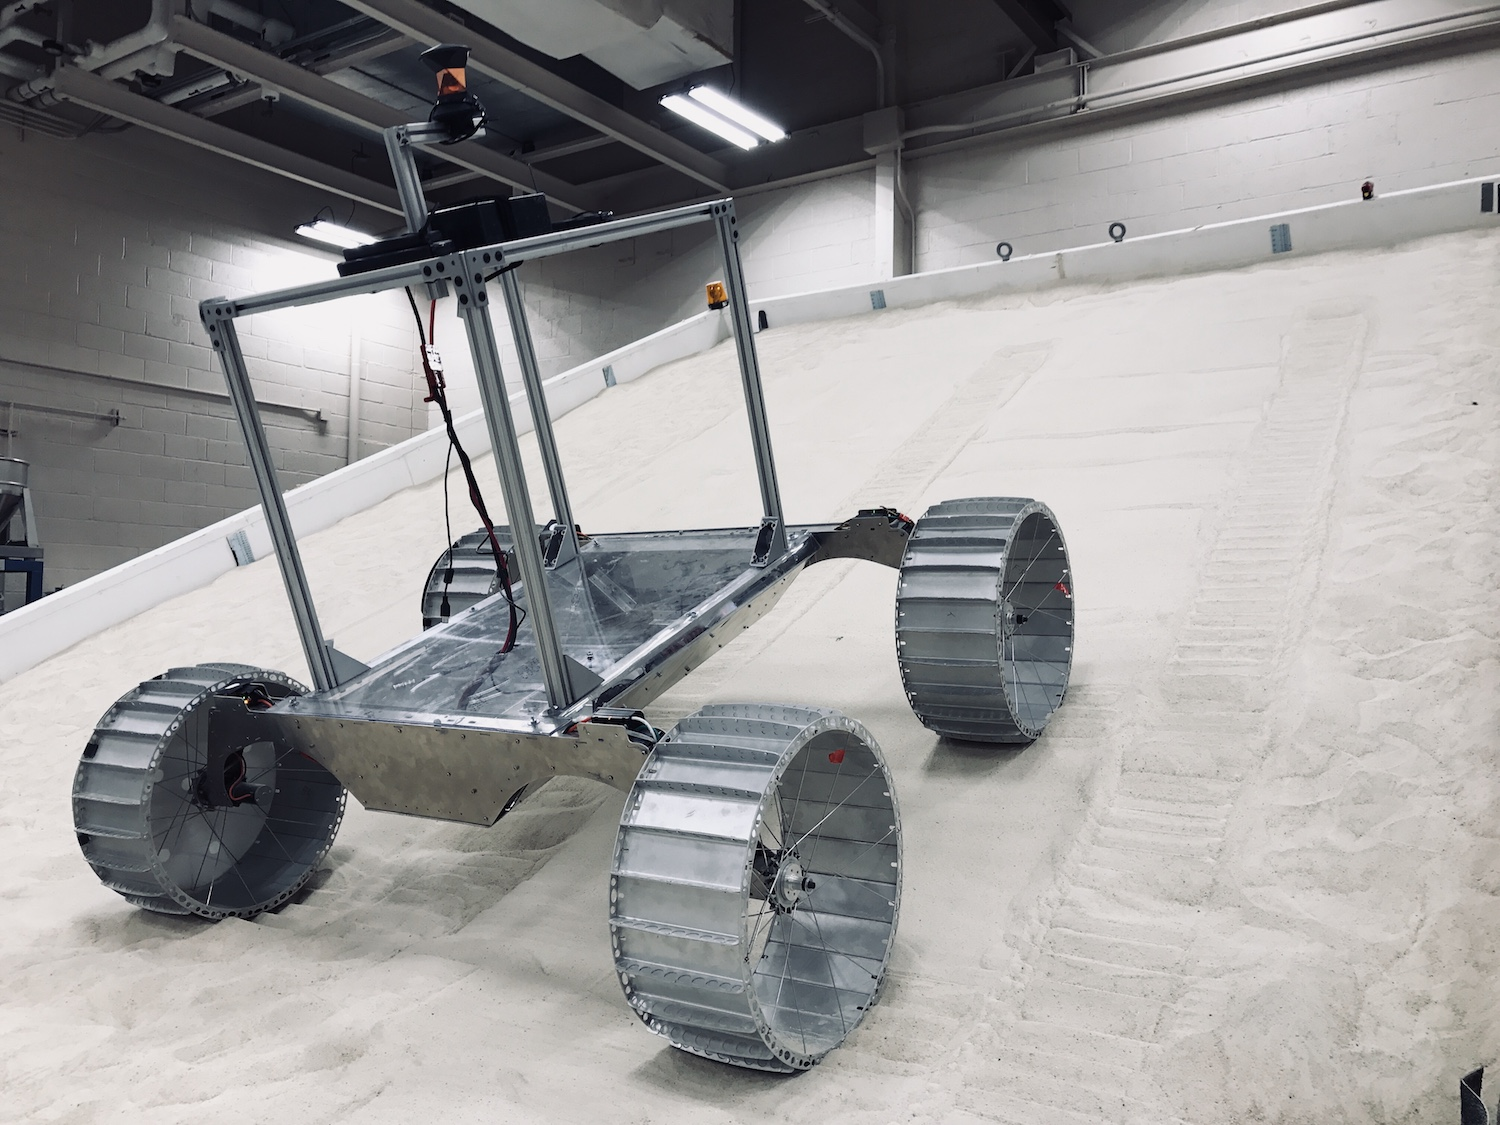
\includegraphics[width=\columnwidth]{figures/wheel_slip_MGRU.JPG}
   	\caption{A picture of the RP Lunar mass equivalent rover at the SLOPElab in NASA GRC.}
    \label{fig:mgru}
\end{figure}
The slip compliance tuning parameter enables simulation of loose material generating slip greater than zero on shallow angle slopes.

Although not perfect at simulating the wheel/soil interaction, this plug-in enables the simulated rover to have a high level slip behavior relatively close to what will be expected on a Lunar terrain. 
In order to increase the fidelity and give more realism for wheel sinkage and rover embedding, this simple model would need to be replaced by a discrete element method (DEM) model which is very computationally expensive \cite{soni2012dem}. Additionally, existing DEM solutions lack validations for lunar terrain.

%%%%%%%%%%%%%%%%%%%%%%%%%%%%%%%%%%%%%%
\section{Flight Software Prototype}
\label{sec:flight-software}
%%%%%%%%%%%%%%%%%%%%%%%%%%%%%%%%%%%%%%

\todo[inline]{Big point to stress the distributed autonomy system, the ros-rapid bridge helps us test the end-to-end simulation.  Strongly distinguish that this is a novel architecture, the first time we've taken this approach, ROS gave us to the tools to build the system.}

In order to test operations we used a combination of ROS software components and NASA-developed software to build an end-to-end mission simulator.  As illustrated in \cref{fig:rp-software}, we split the software into on-board (Flight) and off-board (Ground) software components.  

\begin{figure*}
\centering
\includegraphics[width=\textwidth]{figures/flight-ground-split.png}
\caption{On the left hand side we include the software modules that would operate on-board the robot.  These include low-level components, including waypoint following and simple pose estimation fusing wheel odometry and the vehicle's IMU.  
On the right hand side of the diagram are the more computationally intensive algorithms, which are proposed to run on the Earth.  Exploiting greater computing resources on the ground lets the robot access algorithms which would not be feasible on on-board radiation-hardened computers. \label{fig:rp-software}}
\end{figure*}

The RP concept of operations committed to human-in-the-loop driving.  The decision to split the software was possible because of the high communications availability between the rover and the Earth.  

Autonomy algorithms (mapping, planning) carry a substantial burden for validation and verification. Operating the higher-level algorithms on the ground as assistive tools, instead of on-board the rover in a decision-making capacity, mitigates the validation and verification burden, enabling faster and more cost-effective deployment and development.


\subsection{Flight/Ground Software split}

As discussed in \cref{sec:background} we divided the rover software into low-level control and safeguarding components, which were deployed on-board the rover (``flight software''), and higher-level autonomy or assistive tools which operated on Earth (``ground software'').  
The division of those software components are given in \cref{fig:rp-software}.   

The role of the rover was played by the modified simulated RP rover, as described in \cref{sec:simulated-rover}.  The flight software consisted of the components that were designated the minimum viable components to complete the mission.  The flight software components include:

\begin{description}
\item[\textbf{Rover Kinematics}] The software that translates vehicle body motion commands into motor commands.  We modelled the Rover Kinematics module with the move\_base\footnote{\url{http://wiki.ros.org/move_base}} module with additional explicit steering control.
\item[\textbf{Mobility}] The mobility module is responsible for closed-loop control on waypoint navigation.  This functionality was also supplied by the move\_base module. 
\item[\textbf{Localization}]  The pose estimation solution which integrated wheel odometry, a star tracker, and the IMU.  We modelled the Localization module with ROS' robot\_localization\footnote{\url{http://wiki.ros.org/robot_localization}} package.
\item[\textbf{Camera/Gimbal Pointing}] The RP navigation cameras and the high-gain antenna are mounted on gimbals on the mast. This module is responsible for closed-loop control of those gimbals.  
In our simulation we have primarily concerned ourselves with camera pointing and not the effects of antenna pointing, although planned improvements to communications system simulation fidelity would take antenna pointing into account.  
\item[\textbf{Wheel, IMU, Gimbal, and Camera I/O}]  These modules responsible for low-level hardware interfaces.  This functionality was supplied by the ros\_control\footnote{\url{http://wiki.ros.org/ros_control}} module.
\item[\textbf{Rover Mode Manager}] This software component is responsible for preventing the robot from executing illegal or unsafe actions, and ensuring that all on-board modules are in the appropriate operating mode.  
While this module did exist on the prototype RP rover, we did not implement it for the simulated rover operations, and as such we did not seek a ROS equivalent.
\item[\textbf{Virtual Bumper}]  The virtual bumper is designed to keep the rover safe from navigation obstacles, as per \cite{matthies1997fast}. 
This module was not implemented in the simulated rover operations. 
The prototype virtual bumper implemented for the RP project is described in \cite{nefian2017structured}, with a simple safeguarding scheme described in \cite{furlong2016safeguarding}.
\end{description}

%\todo[inline]{Confirm statements about virtual bumper are true.} yes its true -Uland

The ground software components represented higher-level software, which integrated data to improve the situational awareness of the rover drivers.  
The particular modules included in the ground software are:

\begin{description}
\item[\textbf{Advanced Localization}]  The advanced localization module integrated the on-board pose estimates with terrain relative navigation, mono- and stereo-scopic visual odometry.  We again used the robot\_localization module to integrate the different sources of motion estimation. We did not implement the terrain relative navigation in this simulated version, however, the extensible nature of the robot\_localization package would make this addition straightforward.
\item[\textbf{Stereo Reconstruction}] Produces a metric reconstruction of the scene from the rover's stereo cameras.  We used OpenCV\footnote{\url{http://wiki.ros.org/vision_opencv}} to perform Stereo Reconstruction.
\item[\textbf{Mapping}] Uses the estimated pose and reconstructed scenes to build DEMs of the Lunar surface.  \todo[inline]{check on what module we're using.}
\item[\textbf{Hazard Detection}] Provides two forms of hazard detection.  The module processes elevation maps to identify geometric hazards to the rover, producing a cost map.  It also would process images to visually identify potential vehicle hazards that may not appear in the terrain geometry. The ROS costmap\_2d\footnote{\url{http://wiki.ros.org/costmap_2d}} module provided this functionality. 
\item[\textbf{Planning}]  The planning module takes goals issued by the drivers and determines a sequence of waypoints which safely navigate the cost map produced by the Hazard Detection model. We used the move\_base module to plan trajectories between waypoints.  
\item[\textbf{Simulator}]  The simulator acted as an assistive tool for the operators, to ensure that the commands being sent to the rover were the commands that were intended.  We used the Gazebo paper with the modifications described in this paper.  
\item[\textbf{Operator Interface}]  The operations interface was provided through two modules.  Direct and immediate control of the rover was accomplished through NASA Ames Intelligent Robotics Group's VERVE software.  Overall missions operations, and plan-level contextual information was provided through the WARP system.  Both of these modules are described in greater detail below, and communicated to the ROS system using a software bridge developed for mission simulation experiments.
\end{description}

%%%%%%%%%%%%%%%%%%%%%%%%%%%%%%%%%%%%%%
\section{Operations Software}
\label{sec:ops-software}
%%%%%%%%%%%%%%%%%%%%%%%%%%%%%%%%%%%%%%

To enable teams of flight controllers to participate in driving simulations and to improve simulation fidelity, we interfaced the rover model with the mission control software intended for RP.  
This consisted of the robot driving software, VERVE, the instrument monitoring displays, LabVIEW, and an integrated mission control software framework (WARP) that provides a wide variety of functions.  
To make these components speak to each other we developed a bridge that translated messages between the different communications protocols used by the operations software and the simulated rover. 
The bridge primarily converted between ROS and the RAPID communications protocol\cite{torres2009rapid} used by some NASA-developed software. 

In addition to protocol translation, the bridge models time delay and jitter to serve as a space comms emulator.  
Each data topic can be assigned either a fixed time delay and/or assigned to a logical data channel with set bandwidth.  
The logical data channels use a token bucket to restrict data flow and data payload size is either taken directly from the ROS message or from a configuration file for cases where ROS payload size is significantly different from its flight counterpart. 


\subsubsection{VERVE}

The rover driving software is based on the NASA Visual Environment for Robotic Virtual Exploration (VERVE) \cite{lee2013reusable}. VERVE provides an interactive 3D user interface for remote monitoring and commanding of robotic systems (\cref{fig:verve-mvp}) and has been used for several Lunar analog field tests \cite{deans2009robotic} \cite{fong2010robotic} as well as commanding robotic assets from the International Space Station \cite{bualat2013surface}.

\begin{figure*}[htp]
\centering
\includegraphics[width=\textwidth]{figures/verve_mvp.png}
\caption{VERVE was used as the robot control interface for the Mojave Volatiles Prospector (MVP) project.  MVP tested high-tempo prospecting operations which would be applicable to missions like Resource Prospector.}
\label{fig:verve-mvp}
\end{figure*}

\subsubsection{LabVIEW and WARP}

LabVIEW\cite{labview2018} is commercial software and was used during the development and testing of RP's instruments.
The simulation provides inputs that flows through the real data processing pipeline and into the LabVIEW displays (\cref{fig:labview}).

\begin{figure}[h!]
  \includegraphics[width=\columnwidth]{figures/labview.png}
  \caption{Instrument LabVIEW displays}
  \label{fig:labview}
\end{figure}

WARP \cite{trimble2016open} provides a wide-variety of displays needed by flight control teams including real-time and historical telemetry display, caution and warning and event display, access to telemetry dictionaries, shift logs, timelines and activity plans, support for multiple missions, and base maps and map layers including the rover's path and heat map displays of instrument data (\cref{fig:warp}).
WARP is built on OpenMCT \cite{OpenMCT}, a web-based framework developed by NASA’s Advanced Multi-Mission Operations System (AMMOS), Ames Research Center (ARC) and the Jet Propulsion Laboratory (JPL) and is used by several JPL missions including the next Mars rover (M2020).

\begin{figure}[h!]
  \includegraphics[width=\columnwidth]{figures/warp.png}
  \caption{Web-based mission control displays (WARP/OpenMCT).  Figure shows one among many display pages available.}
  \label{fig:warp}
\end{figure}

\subsection{Science Simulation and Software}

The goal of Resource Prospector was to take measurements to estimate the water content at and under the Lunar surface over a 2500 square meter area and to repeat this data collection in several areas that differ by temperature profile.  
This is the scale over which water would be mined to support a potential, future Lunar base.  
The real-time monitoring of instrument data had two purposes.  
The first was to ensure the quality of the data collection and to adjust or correct instrument settings quickly to that end.  
The second was to make tactical decisions about where data collection time was best spent, because the total mission duration available to a solar powered rover at polar sites does not allow a completely methodical data collection pattern.

\subsubsection{World Model}
The science simulation consists of a world model and several instrument models.  
The world model describes the 'truth' that RP was intended to estimate in the form of several interrelated physical quantities that are measured by RP's instruments.  
Two of the instruments, NSS and NIRVSS, were introduced above.  
NSS measured hydrogen concentration in the regolith immediately in front of the rover, and NIRVSS measured surface frost, minerology, and the concentration of ices in regolith brought up by the drill.  
NIRVSS also contained a Longwave Calibration Sensor (LCS) that measured surface temperature.

The world model provides data for these instruments that varies as the rover moves in ways that must be consistent with physics and with theories about how ices have been emplanted or removed.  
It did this by modeling the distribution of several physical quantities, some as 2D functions (variation over the surface) and others as 3D functions (variation within the top meter of regolith).

The quantities modeled are: (a) the surface temperature, (b) the area concentration of water ice as a surface frost, (c) the area concentration of \ce{OH} adhered to the surface, (d) the thickness of the upper layer of regolith that must be dry based on its known thermal history, (e) the water ice concentration in the layer below that as a weight percentage, (f) the volumetric concentration of hydrogen in hydrogen-bearing minerals, and (g) the surface distribution of several minerals.  
The most important of these were the water ice surface and volumetric concentrations.  
The others were included to present a consistent picture and to provide realistic sources of noise and other variations that could make interpreting the data more difficult.

The 2D and 3D functions implemented as a set of 30720 x 30720 arrays generated before simulation and representing a 4cm grid covering a 1.5 km2 area that would be driven over during the simulations.  
This approach was used because the distributions of the quantities (except the minerals) were generated by modeling the physical processes that could have created them over time.  
(The mineral concentrations were modeled as perlin noise.)

A sequence of arrays was generated, with each array calculated using only the arrays before it.  
The DEM was first, followed by the lightmap and then the surface temperature.  
Regolith is an excellent insulator, so the surface temperature can be approximated as a function of sun angle and shadows (ignoring Earthshine and heat rising from the interior).  
Since the DEM was synthetic, the locations and sizes of the craters was known.  
\ce{OH} concentration is modeled a function of surface temperature.  
The thickness of the dry layer is a much more complex function of the time history of the surface temperature, and Earthshine, heat rising from the interior and the exchange of infrared energy between nearby parts of the surface (crater interiors) very much do need to be modeled; this array came from published work\cite{siegler2015}. 
The volumetric distribution of water ice was inspired by a model of impact gardening published in \cite{hurley2012} and is a function of the distance to the rim of nearby craters above a certain size.  
Surface frost only occurs in permanent shadow and its concentration is a function of the contiguous area of each frost patch.  
The mineral concentrations were modeled as perlin noise and could have been calculated at simulation time, but they were converted into arrays to keep the implementation more uniform.  
\cref{fig:data-layers} shows several of these arrays.

\begin{figure*}[htp]
\begin{subfloat}[Surface Temperature]{
\includegraphics[width=0.2\linewidth]{figures/site-model-surface-temp.png}
}
\end{subfloat}
\qquad
\begin{subfloat}[Depth of dry layer]{
\includegraphics[width=0.2\linewidth]{figures/site-model-ice-stability-depth.png}
}
\end{subfloat}
\qquad
\begin{subfloat}[Subsurface Ice Concentration]{
\includegraphics[width=0.2\linewidth]{figures/site-model-weh.png}
}
\end{subfloat}
\qquad
\begin{subfloat}[Surface Frost]{
\includegraphics[width=0.2\linewidth]{figures/site-model-frost.png}
}
\end{subfloat}
\caption{Data layers describing what instruments could see as the rover drives
\label{fig:data-layers}}
\end{figure*}

\subsubsection{Instrument Models}
During simulation, the rover's location was looked up in these arrays and the results were broadcast at several Hz to the instrument models.  
The instrument models added noise and converted these quantities into the data format generated by the sensors within the instruments.  
This allowed most of the real data processing pipeline for each instrument to be used.

\subsubsection{Science Data Displays}
Instrument data was presented to the scientists using the displays that RP intended to use in flight.  
This involved a combination of LabVIEW displays, which were primarily used by the scientists responsible for the health of the instrument and the quality of the data collection, and a web-based set of displays \cite{OpenMCT} that were primarily used by scientists responsible for data interpretation and tactical decision-making.  
(Both kinds of displays were used by both groups.)  The web-based displays presented the most important information available in the LabVIEW displays and also presented instrument data as heat maps on top of 2D site maps so scientists could see how the data was distributed spatially.  
This followed the approach of xGDS \cite{lee2013reusable} and xGDS components would have been used during flight.  \cref{fig:labview} and  \cref{fig:warp} show examples of these displays.

%%%%%%%%%%%%%%%%%%%%%%%%%%%%%%%%%%%%%%
\section{Experiments}
%%%%%%%%%%%%%%%%%%%%%%%%%%%%%%%%%%%%%%

\subsection{Stereo Visual Odometry}
One of the goals of the visual simulation was to provide realistic data for algorithmic development. An example is the stereo visual odometry we implemented for Resource Prospector's ground software to aid in navigation.
Our approach generates 3D point clouds from successive stereo camera images, aligns them using the Point Cloud Library's implementation of the Iterative Closest Point algorithm, and uses the transforms between point clouds to track changes in the rover's movements. This module interacts with other software and sensors to estimate the rover's absolute pose.

To refine the mission's concept of operations, we wanted to know how much overlap is required between camera images for stereo visual odometry to be effective. 
The easiest way to lose overlap between successive images is by yawing the camera or rover, so that is the first test we ran. 
We learned that with camera rotations of 50-degrees or less, stereo visual odometry yields more accurate results than the fused wheel and star tracker odometry we had been using (shown in \cref{fig:odom_error}).

\begin{figure}[h!]
	\includegraphics[width=\columnwidth]{figures/rotating_clouds_with_odom_error.png}
    \caption{Position error vs. camera rotation angle for stereo visual odometry and wheel-and-star-tracker odometry}
    \label{fig:odom_error}
\end{figure}

There are occasionally incorrect point cloud alignments, informing the need to improve performance or to estimate alignment quality for rejection.
It is important to note the results for stereo visual odometry are preliminary; however, our simulator has provided the only opportunity to develop and test such modern robotic approaches with any confidence - Apollo surface images being non-digital and terrestrial analogs being unrealistic.   
There are further tests to run and improvements to be made to both our visual simulation and visual odometry. 
For example, after a specific camera is chosen for the mission we will be able to refine our camera simulation. 
This will affect point cloud generation and require us to run these tests again.

We also learned that using rover lights in shadowed areas hurts our visual odometry results. 
As expected the quality of our stereo point clouds is greatly reduced when the light sources are near the cameras because the Hapke reflectance model simulates strong, contrast-reducing backscatter. 
We have not attempted to quantify results in this area as it is still considered ripe for refinement.

\subsection{Wheel Slip}
\todo[inline]{mallan: add a bit more explanation here}
In order to characterize the \texttt{wheel\_slip\_plugin}, we set up a test harness to gather data on wheel slip behavior over multiple runs. 
We created a Gazebo world with ramps from 0 to 30 degrees at 2 degree increments (see figure \ref{fig:simulationramps}). 
A rostest script would spawn the rover at the base of each ramp and command it to drive 10 meters forward.
Wheel slip was measured by comparing dead reckoning distance driven to ground truth and test runs covered sets of parameter values for longitudinal compliance, physics engine solver iterations, and drive speed. 
\begin{figure}[h!]
	\includegraphics[width=\columnwidth]{figures/world_lots_o_ramps.jpg}
   	\caption{Gazebo simulation for the slip vs slope test with the RP rover.}
    \label{fig:simulationramps}
\end{figure}

Overall, the \texttt{wheel\_slip\_plugin} demonstrated the expected behavior and compared favorably with physical testbed results as can be seen in figure \ref{fig:wheelsliptuningchart}, which compares wheel slip measured from MGRU with the  \texttt{wheel\_slip\_plugin}. 

\begin{figure}[h!]
	\includegraphics[width=\linewidth]{figures/wheel_slip_roverslip2.png}
   	\caption{Comparison of the RP Lunar mass equivalent rover slip on GRC-1 simulant and RP rover slip in the Gazebo simulator.}
    \label{fig:wheelsliptuningchart}
\end{figure}

However, our test results show that at certain angles and compliance values, there is a wide variation in measured wheel slip (see figure \ref{fig:slipdisparities}). Those disparities are particularly large on a flat terrain.
\begin{figure}[h!]
	\includegraphics[width=\linewidth]{figures/slip_compliance_longitudinal.png}
   	\caption{Graph of the slip of the RP rover in Gazebo showing the disparities in the amount of slip.}
    \label{fig:slipdisparities}
\end{figure}

%%%%%%%%%%%%%%%%%%%%%%%%%%%%%%%%%%%%%%
\section{Conclusion}
%%%%%%%%%%%%%%%%%%%%%%%%%%%%%%%%%%%%%%

This project represents a fusion of COTS, open-source software, with domain specific knowledge that resulted in the production of a high-fidelity Lunar rover driving simulation. 
It presents an approach to rapidly developing visual and physical simulations that enable the holistic evaluation of a mission, from concept of operations to algorithm and mechanism design.

The simulator permitted us to develop and test three major areas for the mission operations.  
First, we were able to simulate the physical environment the robot would be operating in.  
This includes medium fidelity wheel/terrain interactions and high fidelity visual simulation of the moon.  
Second, due to the increased physical verisimilitude, we were able to test rover navigation and perception algorithms on the simulation data with increased confidence in the accuracy of the results.  
Third, by virtue of being a high-fidelity simulation of rover mechanism and software behaviour, we were able to close the loop for the communications and operations infrastructure for the mission. 
 Then we were able to test different concepts of operations, and even rover configurations rapidly, and build confidence in the mission design.


\bibliographystyle{unsrt}
\bibliography{refs}


\end{document}
